\chapter{Path planning}
We're using a path planner based on dynamical systems from Albin Dahlin.
The theory is amazing and super interesting, the results are phenomenal.
However, the purpose of the project, we only need to know how it works to tune it.
From the standpoint of control, it already works well enough to be tested in simulation.

Another important point is that replanning is real-time (about 200Hz). Thus,
we can count on the beginning of the path to always coincide with the origin of 
whatever it is we're planning for. This assumption is used in path-following control.

\section{[TODO: expand a bit] Starshaped planner}
The path is a limited-horizon orbit of a dynamical system describing the flow towards the goal:
\[
\dot{r} = M(r, \mathcal{O}) (r^g - r)
\]
where $r$ is the current robot position, $r^g$ the desired goal, $M(\cdot,\cdot)$ a matrix that describes the attractive dynamics, and $\mathcal{O}$ is the set of world obstacles.

\begin{figure}[t]
    \centering
    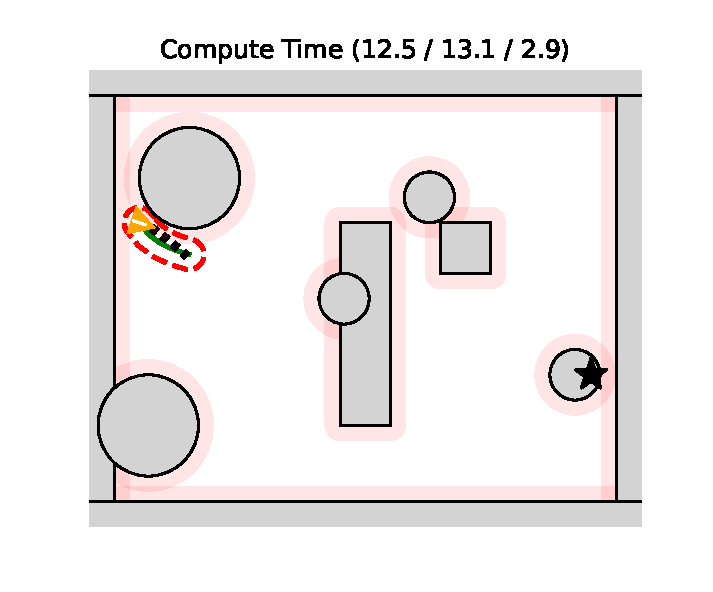
\includegraphics[trim=30 30 30 30,clip,width=0.240\linewidth]{../imgs/08_path_planning/path_1.pdf}
    \hfill
    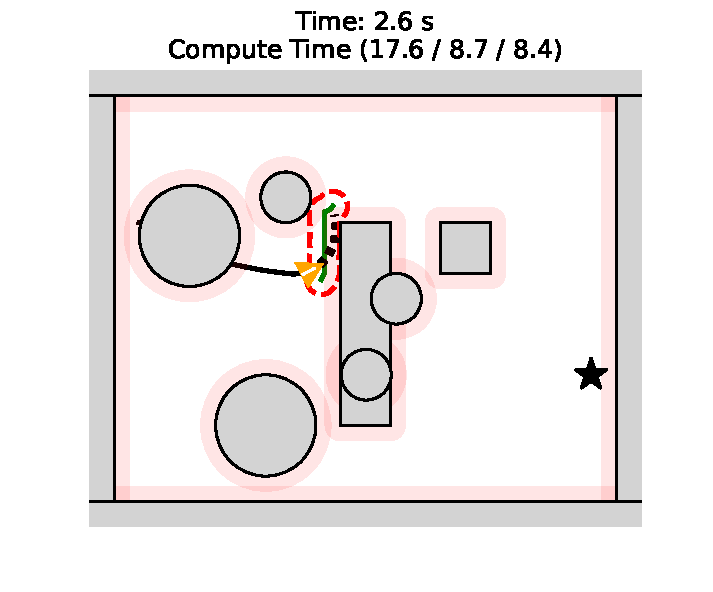
\includegraphics[trim=30 30 30 30,clip,width=0.240\linewidth]{../imgs/08_path_planning/path_2.pdf}
    \hfill
    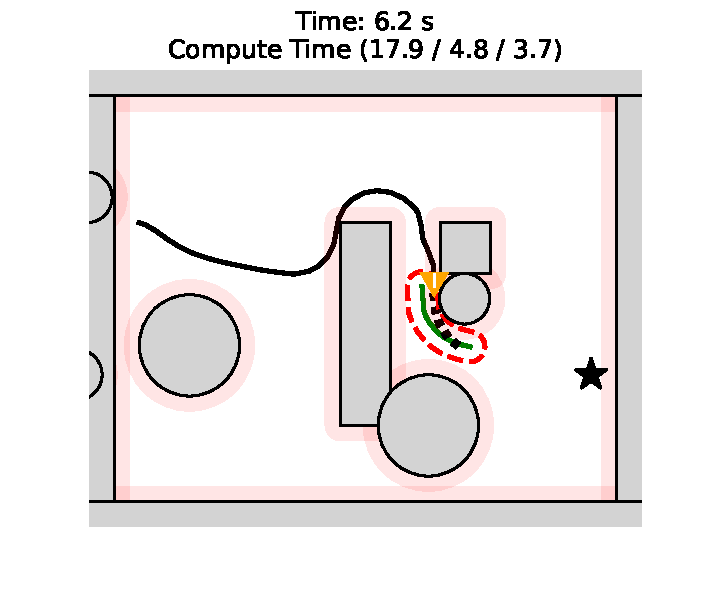
\includegraphics[trim=30 30 30 30,clip,width=0.240\linewidth]{../imgs/08_path_planning/path_3.pdf}
    \hfill
    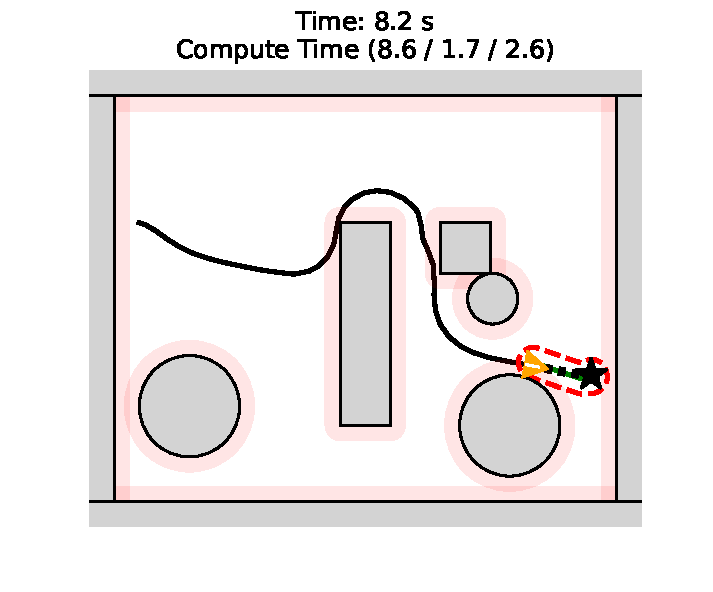
\includegraphics[trim=30 30 30 30,clip,width=0.240\linewidth]{../imgs/08_path_planning/path_4.pdf}
    \caption{Path generation for a unicycle robot with dynamic obstacles and safety guarantees over time (left to right). The robot (yellow arrow) follows the kinematically constrained trajectory (black dashed) while staying inside the safe area (red boundary) of the local desired trajectory (green solid), reaching the goal (star), never colliding with the dynamic obstacles (circles, translating vertically or horizontally). The overall motion is depicted in solid black, while the obstacle safety boundaries are depicted in light red. Generated with \lorem{[Dahlin]}.}
    \label{fig:path_generation}
\end{figure}


\section{TODO: Simulated map}
TODO: just how it's contructed is relevant, but it's just fixed starified rectangles.


\section{Updating map from sensors}
[TODO: expand a bit]
To navigate the cart-robot system in the environment, an obstacle-free path
must be generated. We achieve this in an online fashion, so to account for
dynamic obstacles. Before creating a path, obstacles must be identified and
converted to a useful representation for the planner. We employ LiDAR scanners
to collect distance measurements of the surrounding environment. Then, we
convert these distances to a point cloud and morphologically inflate the points
into circles in the $xy$-plane. A morphological union is then performed so to
gather circles in bigger blobs, which are then simplified in the interest of
computation time for the next step. The starrification algorithm in
\lorem{[Dahlin]} is used to convert the obstacles in \textit{starshaped}
obstacles, which are then further inflated with a clearance radius using
\lorem{[Dahlin]} to create a \textit{tube-path} that guarantees convergence to
the goal pose using the planner in \lorem{[Huber]}.

